\documentclass[a4paper,10pt]{report}

\def\packagepath{../../../preambule}   % path du package principal
\usepackage{\packagepath/preambule}    % utilisation du fichier de configuration

\def\level{BTS }              % Classe
\def\course{TP -- Dérivation et thermique}           % Matière
\def\eval{\quad }

\def\visibleornot{visible}    % visible or invisible
\def\documentpath{./Sources_Latex}
\def\date{20 février -- 13 mars 2026}
\renewcommand{\arraystretch}{1}  % Ecart dans les tableaux

\def\ptsexoA{0}
\def\ptsexoB{0}

\def\ptstotal{\ptsexoA+\ptsexoB}

\usepackage{hyperref}

\usetikzlibrary{shapes, arrows, positioning}
\usetikzlibrary{shapes.geometric, arrows, positioning, decorations.pathreplacing}

\tikzstyle{etat} = [draw, rounded corners=15pt, minimum width=2.5cm, minimum height=1.2cm, text centered, font=\bfseries]
\tikzstyle{fleche} = [thick, ->, >=stealth]

\usepackage{float}
\usepackage[T1]{fontenc}

\begin{document}

\renewcommand{\labelitemi}{\textbullet}

\pagestyle{DS_FP}
\NomPrenomNote{}

%%=============================================================
\exods{\ptsexoA}

\medskip

\begin{easybox*}{Contexte}{}

Lors de tests en laboratoire, on modélise la \textbf{température} $T$ (en °C) d'un microprocesseur en fonction du temps $t$ (en secondes) après sa mise sous tension par la fonction :

$$f(t)=(at+b)\,\e^{-0{,}3t}$$

où $a$ et $b$ sont deux réels à déterminer.
\end{easybox*}

\bigskip

\begin{easybox*}{Conditions expérimentales :}{}

\begin{itemize}
    \item Au démarrage ($t = 0$), la température mesurée est de \textbf{20 °C} (température ambiante).
    \item La tangente à la courbe représentative de $f$ à l'origine a pour coefficient directeur $\mathbf{4}$ (la température monte rapidement au démarrage).
\end{itemize}

\end{easybox*}

\medskip

\begin{enumerate}
    \item À l'aide de Géogebra et des conditions expérimentales, déterminer les valeurs des paramètres $a$ et $b$ et donner l'expression de la fonction $f$.
    \begin{answer}{1}{1}
        $a= \dotfill$ \hfill $b= \dotfill$ \hfill $f(t)= \dotfill$
    \end{answer}

    \item Montrer que la fonction dérivée de $f$ peut s'écrire sous la forme :
    $$f'(t) = (4-3t)\,\e^{-0{,}3t}$$
    \begin{answer}{1}{3.5} \end{answer}

    \item Déterminer le signe de $f'(t)$ sur $[0\,;\,+\infty[$ et compléter le tableau de variation de $f$.

    \begin{answer}{1}{8}
    \begin{minipage}{0.48\linewidth}
        \phantom{espace pour le raisonnement}
    \end{minipage}\hfill
    \begin{minipage}{0.48\linewidth}
        \begin{center}
        \begin{tikzpicture}
        \tkzTabInit[lgt=2,espcl=3.5]
        {$t$ / 1, $\text{signe } f'(t)$ / 1, $\text{var. } f$ / 1}
        {$0$, $+\infty$}
        \tkzTabLine{}
        \tkzTabVar{}
        \end{tikzpicture}
        \end{center}
    \end{minipage}
    \end{answer}

    \pagebreak
    \thispagestyle{DS_LP}

    \item Déterminer l'équation de la tangente à la courbe représentative de $f$ au point d'abscisse $t = 0$.
    \begin{answer}{1}{4} \end{answer}

    \item La \textbf{température maximale de fonctionnement} du microprocesseur est fixée à \textbf{22 °C}. 
    Déterminer à partir de quel instant la température du composant dépasse cette valeur. On arrondira le résultat à la centième de seconde.

    \begin{answer}{1}{1} \end{answer}
\end{enumerate}

%%=============================================================
\exods{\ptsexoB}

\medskip

\begin{easybox*}{Énergie dissipée par le microprocesseur}{}

On s'intéresse à l'énergie thermique dissipée par le composant. On modélise la \textbf{puissance instantanée dissipée} (en watts) à l'instant $t$ (en secondes) par :

$$p(t) = 5t\,\e^{-0{,}3t}$$

\end{easybox*}

\medskip

Un ingénieur propose que la fonction $G(t)$ représente l'énergie totale dissipée (en joules) depuis $t = 0$ jusqu'à l'instant $t$.

\medskip

\begin{enumerate}
    \item Déterminer une fonction $P$ primitive de la fonction $p$.
    \begin{answer}{1}{5} \end{answer}

    \item Le composant est à l'arrêt à $t = 0$ (aucune énergie dissipée). Déterminer la primitive $H$ de $p$ vérifiant $H(0) = 0$.
    \begin{answer}{1}{3} \end{answer}

    \item Déterminer l'énergie totale dissipée par le microprocesseur au bout de \textbf{20 secondes}. On arrondira le résultat à l'unité près.
    \begin{answer}{1}{1} \end{answer}
\end{enumerate}



\end{document}